\begin{frameExample}{Producción}{}
  % EXAMPLE 2.6-1 (Production Allocation Problem} Gupta ebook
  Una empresa produce tres productos. Estos productos se procesan en tres máquinas diferentes. El tiempo requerido para fabricar una unidad de cada uno de los tres productos y la capacidad diaria de las tres máquinas se detallan en la tabla a continuación.

  {\centering
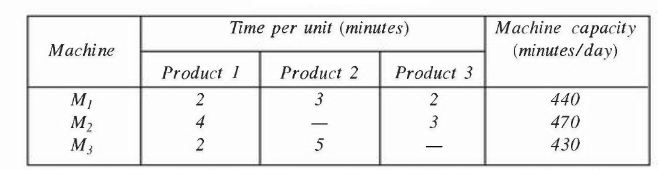
\includegraphics[scale=0.5]{example_allocation_gupta}
\par}

   Se requiere determinar la cantidad diaria de unidades que se fabricarán para cada producto. El beneficio por unidad para el producto 1, 2 y 3 es de \$ 4, \$ 3 y \$ 6 respectivamente. Se supone que todas las cantidades producidas se consumen en el mercado. Formule el modelo matemático (L.P.) que maximizará la ganancia diaria.
\end{frameExample}



%%% Local Variables:
%%% mode: latex
%%% TeX-master: "../slides"
%%% End:
